\documentclass[12pt,english]{article}
\usepackage{geometry}
\geometry{verbose, letterpaper, tmargin = 2.54cm, bmargin = 2.54cm,
  lmargin = 2.54cm, rmargin = 2.54cm}
\geometry{letterpaper}
\usepackage{graphicx}
\usepackage{amsmath}
\usepackage{setspace}
\usepackage{url}
\usepackage{lineno}
\usepackage{xcolor}
\renewcommand\linenumberfont{\normalfont\tiny\sffamily\color{gray}}
\modulolinenumbers[2]

% Linux Libertine:
\usepackage{textcomp}
\usepackage[sb]{libertine}
\usepackage[varqu,varl]{inconsolata}% sans serif typewriter
\usepackage[libertine,bigdelims,vvarbb]{newtxmath} % bb from STIX
\usepackage[cal=boondoxo]{mathalfa} % mathcal
\useosf % osf for text, not math
\usepackage[supstfm=libertinesups,%
  supscaled=1.2,%
  raised=-.13em]{superiors}

\textheight 22.0cm

\usepackage[round,sectionbib]{natbib}
\bibpunct{(}{)}{;}{a}{}{;}
\bibliographystyle{mee}

\title{Modelling spatiotemporal extremes in ecology}
\author{
Sean C. Anderson$^1$ and
Eric J. Ward$^2$
}
\date{}

\begin{document}

\maketitle

\begin{spacing}{1.05}

\begin{abstract}

Understanding biological responses to environmental perturbations in time and
space is critical for conservation planning. With projected trends in climate
forcing, for example, conservation biology will have to focus not just on mean
changes, but also on variability and extremes. In ecological systems, extremes
can happen in time, such as population crashes, or in space, such as rapid
range contractions. Here, we introduce a statistical model that extends current
methods for joint inference about temporal and spatial dynamics (spatiotemporal
modelling) to allow for and detect extremes that occur simultaneously in time
and space. Specifically, our model is a Bayesian predictive-process model that
uses a multivariate-t distribution to describe spatial random effects. The
model is easily implemented with our flexible new R package \textbf{rrfields},
which uses an interface that should be familiar to anyone who has worked with
regression in R. We illustrate applications of our model and R package simulated and
real-world data. First, we \ldots
Second, we predict tree mortality from mountain pine beetle (\emph{Dendroctonus
  ponderosae}) outbreaks in the US Pacific Northwest over the last 16 years. In
both cases, we show that our model provides more accurate and certain
predictions of these ecological processes compared to traditional
spatiotemporal models that do not allow for extremes. Jointly modelling
ecological processes in time and space represents an important step forward to
creating realistic models of anomalies, and allows us to improve predictions
that feed into conservation decisions. Distributing this tool as an R package
should make these models accessible to a wide range of conservation biologists
and scientists in other disciplines interested in predicting extreme events.
\end{abstract}

\section{Introduction}

Applications of statistical models that allow for joint inference about spatial
and temporal dynamics have advanced rapidly in ecology over the last several
decades \citep{bascompte1995, latimer2009}. Spatiotemporal models have also
been widely used in other disciplines, including applications to weather,
remote sensing, human disease dynamics, and crime \citep{cressie2011}. Many
types of linear and non-linear models that ecologists are accustomed to working
with (e.g.~generalized linear models, generalized additive models) can be
modified to include spatiotemporal components, where spatial processes are
modeled as multivariate random effects. Many of these methods are available in
existing R packages, including but not limited to \textbf{spBayes}
\citep{finley2007}, \textbf{spTimer} \citep{bakar2015}, \textbf{INLA}
\citep{rue2009}, \textbf{RandomFields} \citep{schlather2016}, and
\textbf{spate} \citep{sigrist2015}.

For large datasets that include more than several hundred spatial locations,
estimation of multivariate random effects at the locations of the data may be
computationally prohibitive. One solution to this dimensionality problem is to
estimate the random field as correlated random effects at a smaller subset of
locations or $m$ `knots' \citep[e.g.][]{latimer2009, shelton2014}, where $m
  < n$, the number of data points. The estimated random effects are assumed to
be jointly distributed (e.g.~multivariate normal). Instead of estimating an
unconstrained $m \times m$ covariance matrix, a covariance function is
specified \emph{a priori} to estimate the covariance between locations; this
function may be isotropic (where covariance is a function of distance,
e.g.~exponential or Gaussian) or anisotropic (where covariance also depends on
direction, e.g.~Matern). Given the estimated random effects at the knot
locations, and the known distance matrix between the knots and observed data,
it is straightforward to project or interpolate those random effects to the
locations of observations \citep{latimer2009, finley2009}.

Reducing the spatial dimension of a dataset yields a smaller covariance matrix,
but may still be computationally intensive because the covariance matrix is
dense (most elements are non-zero). For some spatial problems, inference about
the covariance between points separated by large distances may not be of
interest because the correlation is negligible. In geostatistics, the `range'
of a semivariogram is often used to identify thresholds beyond which pairs of
points are not correlated \citep{rossi1992}. A second approach to increase the
efficiency of parameter estimation in spatiotemporal models with large datasets
is to implement models that rely on sparse matrix algorithms. One of the most
recent advances in these class of models is the stochastic partial differential
equation (SPDE) approximation to Gaussian random fields proposed by
\citet{lindgren2011}. These methods have been implemented using the integrated
nested Laplace approximation (INLA) \citep{rue2009}, which allows for
approximate Bayesian inference without Markov chain Monte Carlo (MCMC)
sampling. Use of the SPDE-INLA approach has increased rapidly in ecology over
the last five years \citep[e.g.][]{illian2013, ono2016}.

A limitation of models that include Gaussian random fields is that they may
perform poorly when underlying data include anomalous or extreme events. More
on dragon kings and stuff here? Extreme events in temporal processes have been
modeled using a variety of methods in ecology, typically by including finite
mixtures of normal and
heavy-tailed distributions \citep{everitt1996, ward2007, thorson2011}.
More recently, the use of the Student-t distribution
has been proposed as a robust solution to modeling process variation in
population dynamics (Anderson et al. in press).

Several robust extensions of Gaussian random fields have been proposed to
better model extreme spatial events, including applications of max-stable or
extreme value theory \citep{davison2012, davison2012a}. Many of the
applications of these models, such as understanding extremes in rainfall or
flooding, are interested in quantifying the probabilities of exceeding some
threshold \citep{davis2008}. Other extensions of spatiotemporal models to model
extremes include the use of multivariate-t spatial random fields
\citep{roislien2007}. Focusing on the latter, to our knowledge these methods
have not been considered for data in the ecology, fisheries, or environmental
sciences.

The objectives of this paper are to introduce the use of robust spatial
predictive models using the multivariate-t distribution, easily implemented in
our new R package \textbf{rrfields} (robust random fields). Using simulation
testing to compare the multivariate normal to multivariate-t spatial processes,
we illustrate that the multivariate-t leads to better prediction (less bias,
lower uncertainty). Second, we illustrate applications of these modeling
approaches to real-world data that include spatial extremes, using chlorophyll
data from the west coast of the United States \citep{mckibben2012}, and counts
of European starlings (\emph{Sturnus vulgaris}) from the North American
Breeding Bird Survey \citep{pardieck2016}. These applications differ in their
observation error model (normal, Gamma) and treatment of temporal change,
illustrating the flexibility of these robust spatial models to other
applications in ecology and related fields.

\section{Methods}

\subsection{Simulated data}

To evaluate the utility and limitations of spatiotemporal models with
multivariate-t spatial predictive models, we first simulated spatial data and
evaluated our ability to recover the known simulation parameters. Each
simulated data set was generated with data collected at 
100 random locations, and consisted of
$n_t$ replicates in time (e.g.~simulated years). 
We used the random locations for each dataset 
and the partitioning around medoids algorithm
\citep[\texttt{pam()} in the R package \textbf{cluster};][]{reynolds2006}
to calculate the location of knots. The locations of the data were constant
through time such that simulated survey locations (or locations of knots) did
not vary through time.

We used a Gaussian covariance function to model the correlation between
locations because this is one of the most commonly adopted covariance functions
for spatiotemporal models. The Gaussian function (also known as the squared
exponential) models the correlation between points $i$ and $j$:

\begin{equation}
H(\delta_{ij}) = \exp \left(-\phi \delta_{ij}^2 \right)
\end{equation}

and the elements of the covariance matrix at the \emph{m} knot locations:

\begin{equation}
\Sigma_{ij}^*=\sigma^2 \left( -\phi \delta_{ij}^2 \right)
\end{equation}

\begin{figure}[htb]
\begin{center}
  \includegraphics[width=0.8\textwidth]{../figs/pp-illustration.pdf}
\caption{caption}
\label{fig:didactic}
\end{center}
\end{figure}

Each element of the covariance matrix $\Sigma^*$ is thus dependent on
three quantities: (1) $\delta_{ij}$ the known distance between points $i$ and
$j$ squared, (2) the scale parameter $\phi$, which determines how steeply the
correlation declines with increasing distance, and (3) the variance $\sigma^2$.
Following \citep{latimer2009}, we can also calculate the covariance matrix
between the locations of the data and the knots, 
$\Sigma_{\left(W, W^* \right)}$. 
Given $\Sigma^*$, we generated random effects at knot
locations by drawing from a multivariate-t distribution for each time step $t$, 
$W_t^*\sim \mathrm{MVT}\left( \Sigma^{*},\nu \right)$ .
These random effects at the knots are then projected to the data locations using
$\Sigma_{\left( W,W^{*} \right)}$ \citep{latimer2009}.
Given ${\Sigma}^{*}$:

\begin{equation}
W=\Sigma_{\left(W,W^* \right)}^{'} \Sigma^{*-1}W^*
\end{equation}
    
A final step in our data simulation was to corrupt the `true' data by
including measurement or observation error. We assumed observations to be
generated from a Gamma distribution, 
$Y_{it}\sim \mathrm{Gamma}\left(a,\frac {a}{E[Y_{it}]} \right)$, 
where the Gamma shape parameter
$a$ can be reparameterized into the coefficient of variation (CV), 
$a=\frac{1}{CV^2}$.

We used the simulation model described above as the estimation model for each
dataset.

We evaluated a range of parameter values \ldots

Sean - more text here on number of simulations, possibly ranges of
parameters, estimation in STAN, etc.

\begin{figure}[htb]
\begin{center}
  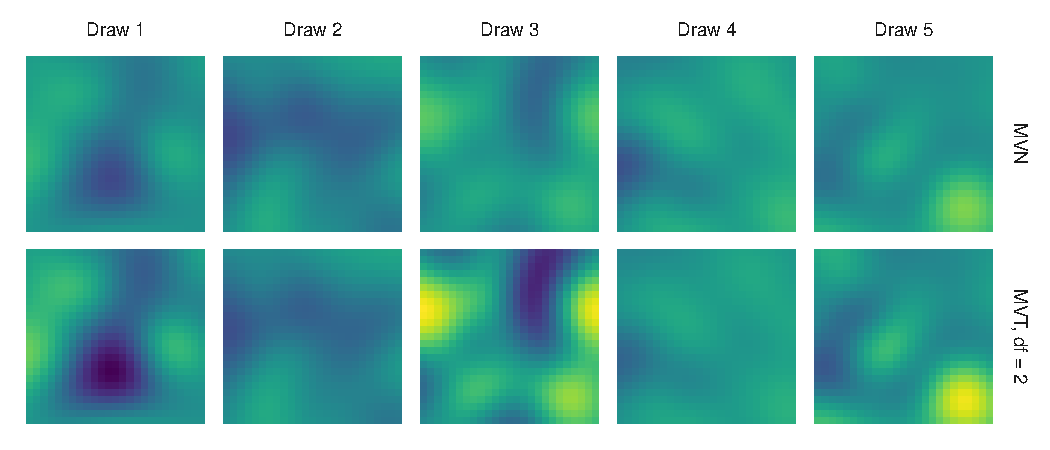
\includegraphics[width=0.9\textwidth]{../figs/nu-rf-illustration.pdf}
\caption{caption}
\label{fig:didactic}
\end{center}
\end{figure}


\subsection{Mountain pine beetles in the US Pacific Northwest}

To illustrate real-world applications of multivariate-t distributed
spatiotemporal models and the rrfields package, 

We fit two spatial models to the data, (1) a model with
multivariate-t random fields and (2) a model with multivariate-normal random
fields. For both models, we expanded on the estimation model applied to
simulated data to include variable random effects by time step (representing
seasonal anomalies in the mean across the entire field). We also assumed normal
residual error, so that the data for location $i$ in time $t$ is
assumed to be 
$Y_{it}\sim \mathrm{Normal}\left(W_{it}+y_t, \sigma \right)$, 
where $W_{it}$ is the estimated random effect
at location $i$ in time $t$, $y_t$ is the intercept for each time
step, and $\sigma$ represents residual error. 
We modeled the temporal intercepts as an autoregressive random walk, 
so that 
$y_t\sim \mathrm{Normal}\left( y_{t-1},\sigma_t \right)$ , and
$\sigma_t$ represents the standard deviation of the temporal intercepts.

Expand on this when we figure out how we're evaluating predictive accuracy

\section{Results}

\section{Discussion}

\bibliography{spatial-extremes}

\end{spacing}
\end{document}
